%!TEX TS-program = xelatex
\documentclass[a4paper]{friggeri-cv}
\addbibresource{bibliography.bib}
\usepackage{graphicx} 
\begin{document}
\header{Alexander }{Müller}
       {}
% In the aside, each new line forces a line break
\begin{aside}
 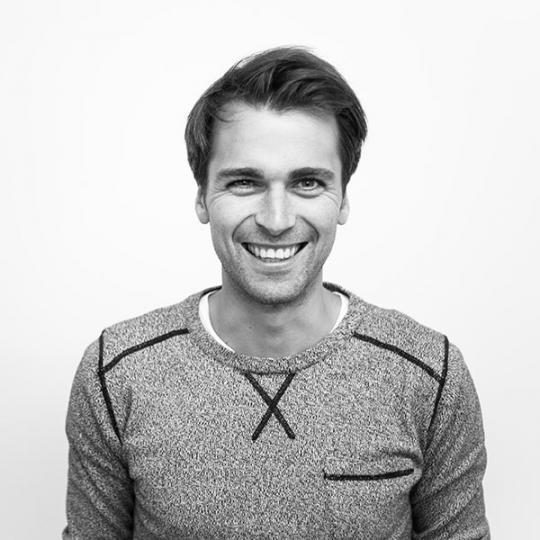
\includegraphics[width=0.9\textwidth]{alex-mueller.jpg} 
  \section{about}
  	born 10th January 1989
  	Gütersloh Germany
  	~
   	Am Lokdepot 3
    10965 Berlin
    Germany
    ~
    \href{mailto:mail@alexcmueller.de}{mail@alexcmueller.de}
    \href{http://alexcmueller.de}{http://alexcmueller.de}
    0176-34557235
  \section{languages}
    native German
    fluent English
    basic Spanish
  \section{programming}
    Python 3
    (Flask, Celery, Airflow)
    Java, Scala
    (Play Framework, Java 8)
    JavaScript
    (Node.js, React)
    NoSQL
    (Cassandra, Redis)
    SQL
    (Postgres, Vertica)
    \section{data analysis}
   	Python (scipy, numpy, sklearn, pandas, xgboost,jupyter)
   	Spark
    Tableau
   	Weka
   	Stanford Core NLP
    \section{hobbies}
    Long-distance running
    Politics
    History
\end{aside}
\section{Work Experience}

\begin{entrylist}
  \entry
    {since 10/2016}
    {Lead Data Scientist}
    {Minodes GmbH, Berlin, Germany}
    {Building and leading a team of 4 data scientist and engineers at Minodes. We are responsible to build new data-driven features and to monitor and improve the data quality of our existing products.}
   \entry
    {06/2015-09/2016}
    {Data Engineer}
    {Minodes GmbH, Berlin, Germany}
    {Data Engineer developing the data processing pipeline enabling WIFI-based offline store analytics, introducing Apache Cassandra and Airflow during this time.}
  \entry
    {since 2016}
    {Freelance Trainer}
    {Various companies in Germany}
    {Conduct digital awareness trainings for german companies to help them to find out about ways to digitize their business models}
  \entry
    {2009-2012}
    {Junior Software Developer}
    {SAP SE, Walldorf, Germany; Montreal, Canada}
    {Worked for different departments during the SAP Study program including SAP Research, CRM Consulting,SAP Predictive maintenance}
\end{entrylist}

\section{Education}

\begin{entrylist}
  \eduentrythesis
    {2012 - 2015}
    {M.Sc. in Business Informatics}
    {University of Mannheim, ITESM Guadalajara(Mexico)}
    {Specialization in Data and Web science, exchange semester in Mexico}
    {Thesis Topic: Towards An unsupervised Ontology Matching System using Outlier Analysis}
    {GPA (GER) : 1,1, ECTS-Rating: A}
  \eduentrythesis
    {2009 – 2012}
    {B.Sc Business Information Technology}
    {DHBW Mannheim in cooperation with SAP SE}
    {Specialization in Software Engineering}
    {Thesis Topic: Design \& Implementation of a Process Mining Application for the Analysis of Weakspots in Business Processes based on In-Memory Database Technology}
    {GPA (GER): 1.4, ECTS-Rating: A}
  \entry
    {until 2008}
    {University Entrance Qualification (Abitur)}
    {priv. Gymnasium Marienschule Lippstadt}
    {GPA (GER): 1.4}
\end{entrylist}


\section{Voluntary activity}
\begin{entrylist}
	\entry
	 {since 2014}
    {Founder and Chairman}
    {Hackerstolz e.v.}
    {Founded Hackerstolz (\href{http://hackerstolz.de}{hackerstolz.de}) as a non-profit association that has the goal to foster the digitize of Germany. Therefore we organize Hackathons and Hackschools.}
	\entry
	 {2015}
    {Organiser}
    {Hackathons}
    {Organized food\{hacks\} (\href{http://food-hacks.de}{food-hacks.de}) and mobility\{hacks\} (\href{http://mobility-hacks.de}{food-hacks.de}) the biggest independently organized hackathons in Berlin that year}
\end{entrylist}


\end{document}
